\section{Introduction}
	\paragraph{}{
	This chapter will outline the implementation process adopted during the project. This will include information on how each component was implemented as well as any issues that occurred during the project and how they were resolved.
	}
\section{Development Environment}{
	\paragraph{}{
	Before starting implementation, a suitable development environment was required. This included a Windows 10 development PC and a method of simulating connection to a vehicle. 
	}
	\paragraph{}{
	A development PC running Windows 10 was required as part of the development environment. It was also preferable that the PC had a touchscreen, to allow testing of gesture controls, such as swipe and pinch, without deploying to a tablet. Fortunately, a Windows 8.1 touchscreen laptop which was eligible for a free Windows 10 upgrade was available before the project began. After the development PC was set up, a suitable Windows 10 tablet to deploy the application on was found. This was a low to middle end tablet, representing what an average user may own.
	}
	
	\paragraph{}{
	In order to be able to test the application, it needed to connect to and communicate with a vehicle. However, this was not practical as it would require moving from the development environment to the vehicle when testing or debugging the application. Initially, an application that simulated connection to an ECU was bought and used. However, during development it became evident that this would not be suitable for the project. Details about the application and why it was not suitable is discussed in section \ref{ssec:SimSoftware}.
	}
	
	\paragraph{}{
	Instead, an ECU test bench was created, shown in Figure \ref{fig:TestBench}, that could be used as part of the development environment. This consisted of an ECU from a Rover 75 with an OBDII port and a power supply. A specific wiring diagram for the ECU had to be acquired in order to connect the wires to the corresponding pins on the ECU and OBDII port. The ECU test bench can be expanded with additional ECUs to facilitate the testing of communications with multiple communication protocols and vehicle manufacturers.
	}	
	
	\begin{figure}[h]
		\begin{center}										
				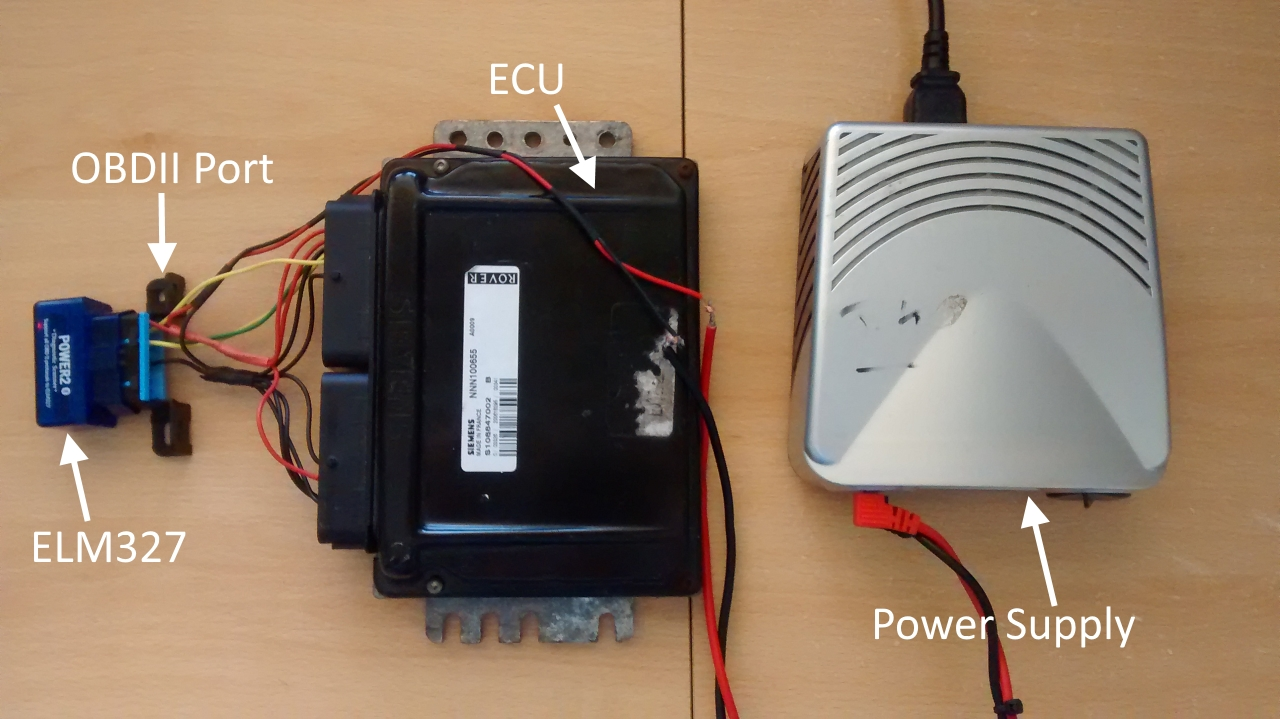
\includegraphics[width=0.8\textwidth]{ECUDesk.jpg}
				\caption{ECU test bench}
				\label{fig:TestBench}
		\end{center}
	\end{figure}
}
\label{sec:DeveEnv}

\section{Prototyping}
	\paragraph{}{
	Prior to starting the project, a lightweight proof of concept was created. This was a C{\#} console application that could connect to an ELM327 simulation application, and display live data on the screen. 
	}
	\paragraph{}{ %Bluetooth API, CAN only
	The application used the 32Feet API by In The Hand Ltd. to handle Bluetooth communication with the ELM327 simulator. The communication system was low level, as it required the address of the laptop and simulator to establish a connection. This was more low level than anticipated and resulted in the hard-coding of the addresses of the development laptop and simulator into the application, which was not optimal. One of the advantages of the 32Feet API, is that the developer can pair Bluetooth devices within their own application. However, this may also be a security issue as an incompatible or harmful device may be paired without the end user's knowledge.
	}
	\paragraph{}{
	The ELM327 simulation software used was an Android application called ECU Engine Pro. The application simulates an ELM327 device connected to an ECU using the CAN protocol. The user can manually add up to six DTCs, and can access the VIN and a limited number of PIDs, such as engine speed. The application displays the address to establish connection via Bluetooth, then the user is taken to the control panel, where they can monitor incoming and outgoing communication logs, as well as edit the DTCs and PID values being returned.
	}
	\paragraph{}{
	The application established communications with the simulator and configured the ELM327 device to use the CAN protocol using the pre-defined commands. The application would then display the first DTC as well as the current engine speed. The values that were displayed were the result of the formatting and converting of the raw data from the simulator.
	}
	\paragraph{}{	
	Overall, the prototype was a success, as it was able to display a DTC as well as the current engine speed on screen. This provided an insight into how communication and data conversion was handled, as well as how to configure the ELM327 device.
	}

\section{Bluetooth Communication}
	\subsection{Description}
		\paragraph{}{
		As the prototype had implemented a subset of the functionality for the communication, it was initially thought that this code could be updated and expanded to create the Bluetooth connection layer. However, during the development process, two key issues became evident, as detailed in section \ref{ssec:BluetoothAPI}. Firstly, the 32Feet Bluetooth API is not supported for UWP applications. Secondly, while UWP applications have their own Bluetooth API, it does not work with the ELM327 simulation software.
		%Implementation of the Bluetooth communication layer of the application began immediately after the setup of the development environment. The goal of this stage was to implement generic Bluetooth communication, such as establishing a connection with the ELM327 device and configuring it, rather than working on module specific communication, such as converting responses. The configuration steps involved resetting the device, allowing the device to auto-detect the communication protocol, turning off echoing of messages and allowing for long responses.
		}
		\paragraph{}{
		Due to these issues, the Bluetooth connection code had to be fully rewritten. This provided some benefits, as the new API is not as low level as the previous one only the device ID is required to establish a connection, rather than the address of the device and the PC. Another key difference with this API is that the developer can not pair devices through the application. Instead, the user has to pair the device manually before using the application. While this was initially viewed as a limitation, it improved the security of the application, as harmful or incompatible devices cannot be paired with the user's PC. Figure \ref{code:BTConnectionInit} shows the connection process, where the Bluetooth service is instantiated using the device ID, which is then used to create a socket to establish communication. A cancellation token is used to timeout the connection attempt after five seconds.
		%not as low level as the previous API, More secure
		}
		
		\begin{figure}[h]
			\begin{lstlisting}
// Set up a service for the Bluetooth device
this.service = await RfcommDeviceService.FromIdAsync(this.CurrentDevice.Id);

if (this.service != null)
{
	this.DeviceConnectionStatus = ConnectionStatus.Connecting;
	this.socket = new StreamSocket();

	// Timeout after 5 seconds
	CancellationTokenSource token = new CancellationTokenSource();
	token.CancelAfter(5000);

	try
	{
		// Connect to the socket
		await socket.ConnectAsync(this.service.ConnectionHostName,this.service.ConnectionServiceName, SocketProtectionLevel.BluetoothEncryptionAllowNullAuthentication).AsTask(token.Token);
	
		// Set up the reader and writer using the socket input stream and output stream respectively
		this.writer = new DataWriter(this.socket.OutputStream);
		this.reader = new DataReader(this.socket.InputStream);    		
	}
	catch(TaskCanceledException e)
	{
		this.DeviceConnectionStatus = ConnectionStatus.NotConnected;                            
	}
}
			\end{lstlisting}
			\caption{Establishing a connection to the ELM327}
			\label{code:BTConnectionInit}
		\end{figure}

		\paragraph{}{
		The main component of the Bluetooth connection system was sending and receiving data. As seen in Figure \ref{code:BTConnectionSend}, a command is sent to the data writer and appended with a return carriage, to inform the ELM327 that the command has terminated. The reader then attempts to read any incoming messages. However, the length of the  message is unknown and can vary for each command. To deal with this, the reader reads one character at a time until a '\textgreater' character appears, signifying the end of the message. If the reader cannot read the entire message, for example, if the user walks out of range of the device, or removes it from the vehicle, the connection will time out.
		% Send & Receive, don't know length of response
		}

		\begin{figure}[h]
			\begin{lstlisting}
// Write
if (this.writer != null)
{
    this.writer.WriteString(command + "\r");
	await this.writer.StoreAsync();
}

// Timeout after 5 seconds                
CancellationTokenSource token = new CancellationTokenSource();
token.CancelAfter(5000);

// Read
try
{
	while (!response.Contains(">"))
	{
		uint size = await this.reader.LoadAsync(1).AsTask(token.Token);                        
        string s = this.reader.ReadString(size);
		response += s;
	}
    
    response = response.Replace(">", "");
}
catch (Exception e)
{
	// Shutdown communication on timeout
	response = NO_CONNECTION;
	this.IsInitialized = false;
}                

if (response.Contains("UNABLE TO CONNECT"))
{
	// Shutdown communication on unable to connect
	response = NO_CONNECTION;
    this.IsInitialized = false;
}

return response;
			\end{lstlisting}
			\caption{Sending a command to the ELM327 and receiving a response}
			\label{code:BTConnectionSend}
		\end{figure}		
		
		%\paragraph{}{
		%There were some issues with the 32Feet Bluetooth API, outlined in section 5.5.1, that lead to the use of Microsoft's own Bluetooth API in it's place. This API allows developers to find all Bluetooth device paired with the PC and choose the appropriate one from the list. Due to the use of this new API, there was less time to work on Bluetooth communication, so the application was created to connect to the first suitable Bluetooth device on the network, with the intention of adding a search function at a later date.
		%}
	\subsection{Issues}
		\subsubsection{Issue 1: Bluetooth API}{
			\paragraph{Description:}
			The 32Feet Bluetooth API used in the prototype was incompatible with the UWP application. This meant that the prototype code that was written for Bluetooth connection could not be reused in the final product.
				
			\paragraph{Occurred during:}
			Semester 1, Week 1
		
			\paragraph{Time taken to resolve:} Half a week to identify the issue, one week to find an alternative solution and one week to implement this solution.
		
			\paragraph{Attempts to resolve:}
			A number of attempts to resolve the issue were made, such as searching for newer versions of the API and researching potential workarounds. Unfortunately, it became evident that the API was completely incompatible with UWP applications, leading to a stand still in development until a replacement could be found.
			
			\paragraph{Solution:}
			Microsoft includes their own Bluetooth API with UWP and this was chosen as a replacement for the 32Feet Bluetooth API. There was an unexpected learning curve that affected the project timeline, but this solution ultimately improved the security of the application and decreased the complexity of the code.
		}
		\label{ssec:BluetoothAPI}
		
		\subsubsection{Issue 2: Simulation software}{
			\paragraph{Description:}
			The replacement Bluetooth API could not connect to the ECU simulation software. This meant connection to an actual vehicle was required to debug and test the application.
			
			\paragraph{Occurred during:}
			Semester 1, Week 1
			\paragraph{Time taken to resolve:}
			One week to find a workaround and half a week to set up the ECU test bench.
			\paragraph{Attempts to resolve:}
			Several attempts to contact the developer were made through emails and the Google Play Store, where the application was bought. Unfortunately, no response was received and a decision was reached that the application could not be utilised for this project, as it seemed highly unlikely that the application would be updated to support the Bluetooth API. 
%Looked for other apps
			\paragraph{Solution:}
			To simulate connection to a vehicle, an ECU test bench was created as outlined in section \ref{sec:DeveEnv}. This had an impact on the timeline of the project, as a number of components, such as an ECU and a wiring diagram, had to be sourced and assembled. Ultimately, the ECU test bench had the advantage of extensibility over the ECU simulation software, as the latter only supported one protocol, whereas the former can be extended with new ECUs that support various protocols.
		}
		\label{ssec:SimSoftware}		

\section{DTC Module}
	\paragraph{}{
	Once the Bluetooth connection system had been implemented, the DTC module was the first component to utilise its functionality. The two key components of this module are retrieving current, pending and permanent DTCs and requesting to clear codes.
	}
	\paragraph{}{
	Initially, the application only retrieved the first current DTC. This provided the opportunity to review the communication process and the look and feel of the user interface. Once the user interface had been finalised, the communication system was updated to retrieve all current DTCs, as seen in Figure \ref{code:DTCModuleCodes}. The process for retrieving DTCs is very similar for each type, with the only difference being the request and response message headers. Because of this, the majority of the code used to retrieve current DTCs could be re-used to retrieve pending and permanent DTCs.
		% Retrieve codes		
	}
	
	\begin{figure}[h]
		\begin{lstlisting}
// Get batches of current codes
string hex = await this.dataConnection.SendCommand("03");

// Split codes into batches
string[] batches = hex.Split('\r');

IList<ICode> codes = new List<ICode>();

foreach (string batch in batches)
{
	// Check if the batch is valid
    if (batch.StartsWith("43"))
    {        
        string codesHex = string.Empty;
        		
		// Remove the header - The CAN protcol uses a longer header
		if (ConnectionManager.Instance.VehicleProtocol == Protocol.CAN)
			codesHex = batch.Substring(4);
        else
			codesHex = batch.Substring(2);

        // Codes are returned in batches of three
		for (int i = 0; i < 3; i++)
		{
			string code = string.Empty;
			code = codesHex.Substring(i * 4, 4);

			// 0000 is not recognised as a valid DTC
			if (code != "0000")
			{
				// The first digit determines the code type (P, C, B, U)
				switch (code.Substring(0, 1))
				{
					case "0": code = "P" + code; break;
					case "4": code = "C" + code; break;
					case "8": code = "B" + code; break;
					case "C": code = "U" + code; break;						
				}					
				
				// Code description is added by the factory
				codes.Add(CodeFactory.CreateCode(code));
			}
		}
       }
}
return codes;
		\end{lstlisting}
		\caption{Retrieving current codes - The same process is used for pending and permanent codes, but with a different header}
		\label{code:DTCModuleCodes}
	\end{figure}
			
		\paragraph{}{
		The second component of this module is the ability to issue the clear codes command. The manner in which this is handled differs greatly from retrieving DTCs. When requesting to clear codes, there is no response that has to be handled. Instead, the application refreshes the list of current DTCs, which will now be empty, thus verifying that the clear codes command was issued.
		% Clear codes
		}
		
		\paragraph{}{
		Unfortunately, due to a number of constraints, additional information for DTCs could not be implemented in the final product. As the project progressed, it became evident that there would not be enough time to gather information on the causes and solutions of each DTC. This was because of the large amount of DTCs, which exceeds four thousand. Some consideration was made for implementing a subset of these DTCs, but given the time frame, it would not be possible to find a reputable source for this information, gain permission for its use and validate the information for all DTCs.
		% DTC Additional Information
		}						
		
\section{Data Module}
	\subsection{Description}{		
		\paragraph{}{
		Implementation for the data module differed greatly as, unlike the other modules, the data module was constantly polling the ECU for information, rather than sending a request once on initialization. The data module is also the most visual of all module as it utilises graphs to display data to the end user.
		%Intro
		}
		
		\paragraph{}{
		The first stage of the data module is compiling a list of supported PIDs. The process for acquiring all supported PIDs is outlined in section \ref{ssec:Data}. However, as seen in Figure \ref{code:SupportedPids}, the data module only acquires the first two sets of supported PIDs, totalling a maximum of sixty four supported PIDs. This was due to the potential performance issues that may arise from rendering too many graphs and also due to the limited timeframe of the project, as it would require conversion code to be written for each PID.
		%Supported pids as outlined in section \ref{ssec:Data}
		%Get supported pids
		}
		
		\begin{figure}[h]
			\begin{lstlisting}
IList<IPid> supportedPids = new List<IPid>();

for (byte i = 0x00; i <= 0x20; i += 0x20)
{
	// Request supported pids
	string request = await this.dataConnection.SendCommand("01" + i.ToString("X2") + "1");

	// Check if the response is valid
	if (request.StartsWith("41"))
	{
		// Remove header
		request = request.Substring(4);

		// Convert to binary
		string binary = Convert.ToString(Convert.ToInt32(request, 16), 2).PadLeft(32, '0');

		// Find all 1s in binary, denoting which pids are supported
		for (int j = 0; j < binary.Length - 1; j++)
		{
			// If the bit is 1, then the pid is supported
			if (binary.Substring(j, 1) == "1")
			{
				// Get the hex value for the pid
				byte hex = i;
				hex += Convert.ToByte(j + 1);
								
				// Create the pid
				string pidHex = hex.ToString("X2");
				IPid pid = PidFactory.CreatePid(pidHex);
				if (pid != null)
					supportedPids.Add(pid);
			}
		}
	}
}
			\end{lstlisting}
			\caption{Get supported pids - Only supports 1000 and 1020}
			\label{code:SupportedPids}
		\end{figure}
		
		\paragraph{}{
		When a request is made, the response that is received is in hexadecimal format. This response contains the header and a number of bytes. To convert this data into a human readable value, a the bytes are passed into a conversion equation. This equation varies for each PID. In Figure \ref{code:ConvertingPids}, the engine speed PID is converted by removing the message header, and passing the response bytes into its conversion equation.
		%[Convert data]
		}
		
		\begin{figure}[h]
			\begin{lstlisting}
public static IDataItem ConvertPID(IPid pid, string request)
{
	// Represent first and second response bytes
	int A, B;
	double value = double.NaN;
	string stringValue = "No Value";
	
	switch(pid.PidHex)
	{
		// Convert response using the equation: ((A * 256) + B) / 4
		case "0C":    
			A = Convert.ToInt32(Convert.ToByte(request.Substring(0, 2), 16));
			B = Convert.ToInt32(Convert.ToByte(request.Substring(2, 2), 16));
			value = ((A * 256) + B) / 4;
			stringValue = value.ToString();
		break;
	}

	IDataItem dataItem = new DataItem(value, stringValue);	
    return dataItem;
}
			\end{lstlisting}
			\caption{Converting Engine Speed PID to human readable value}
			\label{code:ConvertingPids}
		\end{figure}		
			
		\paragraph{}{
		The human readable data values are displayed to the end user in two formats: text and graphs. The text views give a simplified view of each PID, only displaying the current value of a PID. The graph views track all values over a session and plot them so they can be viewed at a later time. The data module also implements controls to play, pause and skip through the values. This allows the user to have full control over what data is presented to them on screen. 
		%[List, Graphs, Play/Pause/Step Controls] 
		}
		
		\paragraph{}{
		The final feature of the data module is the smart graphing system, which is an extension of the existing graphing system. Smart graphing is a system that uses different colour values to represent whether a data value is normal, potentially dangerous or severely dangerous. This system is currently implemented for a subset of pids, due to time constraints and a lack of technical knowledge. As seen in Figure \ref{code:ValueType}, a smart graphing PID is analysed based on its current value and assigned a type. This type determines the colour that will be displayed on the graph.
		%[Smart Graphing]
		}			
		
		\begin{figure}[h]
			\begin{lstlisting}		
private static ValueType GetValueType(IPid pid, IDataItem item)
{
	ValueType type = ValueType.Default;
				
	switch (pid.PidHex)
	{
		case "0C":		
			if (item.Value < 800)
				type = ValueType.Caution;
			else if (item.Value > 5500)
				type = ValueType.Danger;
			else
				type = ValueType.Normal;
		break;

	}
	return type;
}
			\end{lstlisting}
			\caption{Changing the graph colour based on the value}
			\label{code:ValueType}
		\end{figure}		
		
		
		\label{ssec:DataModuleDesc}
	}

	\subsection{Issues}{		
		\subsubsection{Issue 1: Data collection speed}{
			\paragraph{Description:}
			When gathering data samples, it was discovered that the time taken to send a request and receive a response was around 300 milliseconds per request. When a large number of pids are requested, it took around seven seconds per sample.
			\paragraph{Occurred during:}
			Holiday period, Week 1
			\paragraph{Time taken to resolve:}
			Approximately three weeks
			\paragraph{Attempts to resolve:}
			The application was tested with other ECUs and vehicle protocols to see if the issue was with the test bench. A number of attempts were also made to re-factor the Bluetooth communication system. However, these attempts did not see any improvement in performance.
			%[NUM PIDS LIMITED]
			\paragraph{Solution:}
			A solution was found after more research was conducted on the ELM327 device. By default, the device will wait 200 milliseconds before returning a response. To bypass this, the user can pass a numerical parameter with each request, that denotes how many bytes are expected in the response. Once the device has collected this number of bytes, it will skip the waiting period and return the response immediately. This decreased the response time from 300 milliseconds to 170 milliseconds, which was a huge improvement, but the data collection was still slow.
		\subsubsection{Issue 2: Graph blurring}{
			\paragraph{Description:}
			When gathering data samples, the graph plot line started to blur. This blurring became more severe as the number of samples increased. This affected the readability of the data graphs.
			\paragraph{Occurred during:}
			Holiday period, Week 3
			\paragraph{Time taken to resolve:}
			Approximately two weeks
			\paragraph{Attempts to resolve:}
			An attempt was made to cull the graph plot line based on what was visible. However, when this was implemented, it did not seem to fix the issue. 
			\paragraph{Solution:}
			The solution came as part of the implementation of the smart graphing system. Originally, the graph plot was a single line, with a collection of points. In order to add varying colours to the plot line, it had to be split into segments that were coloured individually. By splitting the line into segments, the blurring issue was fixed.
		%[Speed 300ms, down to 170ms]
		%[Graph blurring - Smart graphing fixed this but memory was an issue]
		}
	}
	\label{ssec:DataModuleIssues}

\section{Simulated Communication}{
		\paragraph{}{
		While implementing the data module, a potential problem was discovered. While the ECU test bench sent back data that could be graphed, the values were static and could not be changed. This made it difficult to test the data graphing, as it required communication with a live vehicle to gather dynamic data values. Instead, a simulation connection class was created.
		%[Preparation for data module, acts like an ECU, behaves like real world (time, responses etc)]
		}
		\paragraph{}{
		The simulation connection class implements the IDataConnection interface seen in Figure \ref{code:ConnectionInterface}, but instead of connecting to a Bluetooth device, it handles the requests and returns a response in the format that the ELM327 would use, sending responses in hexadecimal format. Because of this, the simulation connection more accurately represents communication with a vehicle and did not require a refactor of the code in the communication system layer.
		}	
		\begin{figure}[h]
			\begin{lstlisting}
// Default response
string response = "NO DATA";

// Request for Data (Mode 01)
if (command.StartsWith("01"))
{
	// Get supported pids
	if (command.StartsWith("0100"))
    {
		// Binary Value: 0001 1000 0111 1000 0000 0000 0000 0000
		response = "410018580000";
	}
    else if (command.StartsWith("0104"))
	{
    	/* Conversion formula: A * 100 / 255 */
    	
    	// Generate a number between the minimum and maximum value
        int min = 0;
		int max = 100;
        Random r = new Random();
		int value = r.Next(min, max);

		// Reverse the equation and convert to hex
        value = (255 * value) / 100;
		response = "4104" + value.ToString("X2");
	}
}
			\end{lstlisting}
			\caption{Simulation connection code for 0100 and 0104 requests}
			\label{code:SimConnectionData}
		\end{figure}

		\paragraph{}{
		As shown in the code fragment seen  in Figure \ref{code:SimConnectionData}, a small subset of pids are supported, and each of these pids will return data when a request is made. As each PID has a maximum and minimum possible value, a random value between these two will be generated and this will be the value that the user sees on-screen. The value  is passed through a conversion equation, as discussed in section \ref{ssec:DataModuleDesc}, in reverse order to convert it to hexadecimal format. Finally, the response header is prefixed to this hexadecimal message and is returned to the caller.
		}
		\paragraph{}{
		Due to the success of the simulation connection with respect to the data module, it was expanded to work with the DTC module, returning a set of current, pending and permanent DTCs, as seen in Figure \ref{code:SimConnectionDTC}.
		}
	\newpage	
		\begin{figure}[h]
			\begin{lstlisting}
// Current DTCs
if (command.StartsWith("03"))
{
	// Return P0101, P0121 and P0353	
	response = "43010101210353";
}
// Pending DTCs
else if (command.StartsWith("07"))
{
	// Return P0104, P0132 and P0342	
	response = "47010401320342";
}
// Permanent DTCs
else if (command.StartsWith("0A"))
{
	// Return P0107, P0109 and P0111	
	response = "4A010701090111";
}			
			\end{lstlisting}
			\caption{Simulation connection code for current, pending and permanent DTCs}
			\label{code:SimConnectionDTC}
		\end{figure}
\label{sec:Simulation}
}

\section{Connection Module}
		\paragraph{}{
		As discussed in section \ref{ssec:DesignConnectionModule}, the system required a means of selecting an ELM327 device that is paired to the PC. This ensures that the end user has complete control over what device the application uses to communicate with their car.
		}
		
		\paragraph{}{
		The connection module is the first module to be displayed when  the application loads, as the user must connect to a device before using any other modules. If connection to the device is lost while the user is using another module, the application will send the user back to the connection module to reconnect, along with displaying an appropriate message to the user.
		}
		
		\paragraph{}{
		The first component of this module is gathering a list of all Bluetooth devices that are paired	with the PC. Using the UWP Bluetooth API, this is achieved with one method call, as seen in Figure  \ref{code:AvailableDevices}. However, this returns a platform specific Bluetooth devices, which has a negative impact on the portability of the system. To counteract this, the system converts these into a custom device class that contains the name, ID and address of the Bluetooth device. This creates a more portable application, as there is less duplicated code for the Bluetooth communication system.
		}
		%Get paired devices, select one and it connects as outlined in \ref{code:BTConnectionInit}
		%[List of paired devices, connection status, comm log, module is loaded on disconnect]
		}
		
		\begin{figure}[h]
			\begin{lstlisting}
IList<IDevice> availableDevices = new List<IDevice>();

// Get a list of Windows specific Bluetooth devices
DeviceInformationCollection devices = await DeviceInformation.FindAllAsync(RfcommDeviceService.GetDeviceSelector(RfcommServiceId.SerialPort));

foreach(DeviceInformation device in devices)
{
	// Create an instance of custom device class that can be used on all platforms
	IDevice bluetoothDevice = new BluetoothConnectionDevice(device.Name, device.Id, null);
    availableDevices.Add(bluetoothDevice);
}

return availableDevices;
			\end{lstlisting}
			\caption{Finding all available devices}
			\label{code:AvailableDevices}
		\end{figure}
		
		\paragraph{}{
		Once a list of available devices has been gathered, they are displayed on screen as buttons. When the user clicks one of these buttons, the system will attempt to connect to the associated device, using the process seen in Figure \ref{code:BTConnectionInit}. If the connection cannot be established within five seconds, the user will be informed and can retry or select another device.
		}				
		
\section{Android Port}
	\subsection{Description}		
		\paragraph{}{
		A key aspect of the project is the extensibility and portability of the system. To prove this, the system was ported from Windows 10 to Android using the Xamarin framework. Due to time constraints, only a subset of features were made available on Android, but subsequent features can be easily implemented in future iterations.
		%[INTRO]
		}
		\paragraph{}{
		As the project was initially developed as a UWP application, the platform specific code had to be separated from the shared code. The shared code corresponds to the host, module and communication layers in the system, whereas the platform specific code corresponds to the UI and Bluetooth layers. The core code was put into a Portable Class Library (PCL), a library that can be used across multiple platforms, such as Windows 8 and 8.1 applications, WPF applications and applications developed using Xamarin.
		%[PORT PREP + PCL]
		}
		
		\paragraph{}{
		After the preparation was complete, the first stage of porting the system was creating a new Bluetooth layer. Due to the design choices made for the system, this only required one class to be created, that implements the IDataConnection interface, seen in Figure \ref{code:ConnectionInterface}, and utilises the Android Bluetooth API. While there was an initial learning curve, the basic principles of Bluetooth communication are the same, as seen in Figure \ref{code:AndroidBluetoothInit}, that shows the initialization of the Bluetooth connection in the Android application.
		%[BLUETOOTH INIT + CODE]
		}
		
		\begin{figure}[h]
			\begin{lstlisting}
public async Task<bool> Initialize()
{
	this.DeviceConnectionStatus = ConnectionStatus.Connecting;
	
	// Get the Bluetooth adapter and socket
    BluetoothAdapter adapter = BluetoothAdapter.DefaultAdapter;
	this.socket = this.androidDevice.CreateRfcommSocketToServiceRecord(this.uuid);
    
    if(socket != null)
	{
		try
		{
			// Connect to the socket
			await this.socket.ConnectAsync();                           
			await this.Reset();
			this.IsInitialized = true;
		}
		catch(Exception e)
		{
			this.DeviceConnectionStatus = ConnectionStatus.NotConnected;
		}                        
	}
}
			\end{lstlisting}
			\caption{Android Bluetooth Initialize() Method}
			\label{code:AndroidBluetoothInit}
		\end{figure}		

		\paragraph{}{
		There are subtle differences in the Android Bluetooth API, that required more significant changes in the Bluetooth layer during the port. When sending requests and receiving responses, the messages must be sent as byte arrays. This is seen in Figure \ref{code:AndroidBluetoothSend}, where the outgoing string message is converted into a byte array before being sent to the ELM327 device. While it was believed that the new API may be faster and therefore fix the data collection speed issue outlined in \ref{ssec:DataModuleIssues}, this was not the case, as the data collection speed was approximately the same.
		%[BLUETOOTH SEND + CODE]
		}

		\begin{figure}[h]
			\begin{lstlisting}
public async Task<string> SendCommand(string command)
{
    string response = string.Empty;

	// Convert string to byte array
	char[] charArray = (command + "\r").ToCharArray();
	byte[] outgoingMessage = new byte[charArray.Length];
	for (int i = 0; i < charArray.Length; i++)
		outgoingMessage[i] = (byte)charArray[i];

	// Write
	await this.socket.OutputStream.WriteAsync(outgoingMessage, 0, outgoingMessage.Length);

	// Read
	while (!response.Contains(">"))
	{
		byte[] incomingMessage = new byte[1024];
		await this.socket.InputStream.ReadAsync(incomingMessage, 0, incomingMessage.Length);

		foreach (byte b in incomingMessage)
		{
			if (b != 0)
			{
				response += Convert.ToChar(b);
			}
		}    
	}
	return response;
}
			\end{lstlisting}
			\caption{Android Bluetooth SendCommand() Method}
			\label{code:AndroidBluetoothSend}
		\end{figure}
		
		\paragraph{}{
		The second stage of porting the system was creating a new UI layer. Figure \ref{code:AndroidCodeUI} shows the implementation for the DTC Module user interface. As the system utilises MVVM, where the viewmodel notifies of any property changes, the user interface only needs to subscribe to these notifications and perform the relevant actions. In the case of the DTC user interface, the user interface listens for changes to the module viewmodel and redraws the lists of DTCs when it is notified.
		%[UI + CODE + MVVM]
		}
		\begin{figure}[h]
			\begin{lstlisting}
public CodesFragment(IDtcModuleViewModel module)
{
	// Subscribe to the PropertyChanged event handler of the ViewModel
	this.module = module;
	this.module.PropertyChanged += this.RaiseViewModelChanged;
}

private void RaiseViewModelChanged(object sender, PropertyChangedEventArgs e)
{
	// Draw the DTCs on screen when the ViewModel notifies of a change
	this.PopulateCodes();
}			
			\end{lstlisting}
			\caption{User Interface code for the DTC Module}
			\label{code:AndroidCodeUI}
		\end{figure}
					
	\subsection{Issues}{
		\subsubsection{Issue 1: Android emulator not deploying in Visual Studio}{
			\paragraph{Description:}
			The Xamarin framework integrates with Visual Studio and allows Android emulators to be used for deploying applications. These emulators are virtual Android devices that can be used in place of physical devices. However, the application could not be deployed on the emulator.    
			\paragraph{Occurred during:}
			Holiday period, Week 2
			\paragraph{Time taken to resolve:}
			Approximately two weeks
			\paragraph{Attempts to resolve:}
			Research found that other developers had encountered this issue with Visual Studio. The proposed solution was to use Xamarin Studio, an IDE supplied by Xamarin. However, this was not a viable solution, as the time spent switching from one IDE to another when debugging was far greater than deploying to a physical device. 
			\paragraph{Solution:}
			A physical Android device was used to deploy and debug the application. While this was not ideal, it had the benefit of testing a physical device under real world scenarios, rather than a virtual device.
	}
	\label{ssec:AndroidIssues}


\section{Help Information}
		\paragraph{}{
		Once the majority of modules had been implemented, it became clear that the way the modules instructed the end user on how to use them was not optimal. Firstly, these instructions were intrusive and took up valuable screen real estate. This would be an issue when the application is deployed on devices with smaller screens, such as mobile phones. Secondly, over time, the end user will learn to use the application without instructions, at which point the on-screen instructions become redundant.
		%[Moving help info out of other modules, help shouldn't interrupt modules, UI matches on both platforms]
		}
		\paragraph{}{
		A decision was made to re-factor the application so that the instructions were not integrated with the user interface of the module. Instead, the solution was to provide a means of viewing instructions that was separate from the module, but could be accessed without leaving the current module. This was achieved by implementing a pop out window on the right hand side of the screen.
		}
		\paragraph{}{
		The Module interface, shown in Figure \ref{code:ModuleInterface}, was re-factored to include a list of help items, with each help item having a title and a description. As seen in Figure \ref{code:HelpItem}, which shows the implementation of help items for the connection module, the help items are created by a factory method and assigned to a module. The help items are then displayed by clicking the help icon at the top of the screen.
		}
		
		\begin{figure}[h]
			\begin{lstlisting}
public interface IHelpItem
{
    string Title { get; }

	string Description { get; }
}

public class HelpItem : IHelpItem
{
	public string Title { get; private set; }

	public string Description { get; private set; }

	public HelpItem(string title, string description)
	{
		this.Title = title;
		this.Description = description;
	}
}

public static class HelpItemFactory
{
	private static IList<IHelpItem> ConnectionHelpItems()
	{
    	IList<IHelpItem> connectionHelpItems = new List<IHelpItem>();

		connectionHelpItems.Add(new HelpItem("What device do I need?", "You will need an ELM327 Bluetooth device (version 1.3 or later)"));
        connectionHelpItems.Add(new HelpItem("Setup", "1) Enable Bluetooth on your PC / tablet\n" +
                                                          "2) Pair the ELM327 device with your PC / tablet / phone in your device settings\n" +
                                                          "3) Select your ELM327 device from the device list"));

    	return connectionHelpItems;
	}	
}
			\end{lstlisting}
			\caption{Help item interface and an example of how they are implemented for the connection module}
			\label{code:HelpItem}
		\end{figure}
	\newpage
\section{Home Module}
		\paragraph{}{
		The home module is the least technical of all the modules in the system. It serves as a means of teaching users how to utilise the various functions of the application. The user can find a list of functions that are available to use, as well as how and when to use them. This helps to guide new users on where to start when they first load the application.
		}
				
		\paragraph{}{
		The module displays disclaimer information, warning the user not to attempt any repairs on their vehicle and to always seek the advice of a mechanic after using the application. This ensures that the user is aware that the application is used for preliminary diagnosis rather than formal diagnosis.
		}
		

\section{Email}
		\paragraph{}{
		The final feature of the application to be implemented was the email system. This system captures useful data from a module and compiles it into an email so the user can send it to their mechanic. This allows end users to receive a preliminary diagnosis from a person with technical knowledge before they physically travel to a garage for formal diagnosis.		
		%[INTRO]
		}
		\paragraph{}{
		The module interface was re-factored to include a formatted message that can be sent by email. Figure \ref{code:EmailCodes} shows the implementation for the DTC module, which iterates through all DTCs that have been found and adds them to the message. The email system was only implemented for the DTC Module as the other non-technical modules do not require aid from a mechanic. The only other technical module, the data module, does require aid from a mechanic, but sending the data values for each PID would not be sufficient information for the mechanic to make a preliminary diagnosis.
		%Codes only, Module refactor
		}

		\begin{figure}[h]
			\begin{lstlisting}
public string FormatForEmail()
{
	string message = "My vehicle has the following DTCS:\n";

	message += "\nCurrent Codes\n";
	foreach (ICodeViewModel code in this.CurrentCodes)
    	message += string.Format("{0} - {1}\n", code.Name, code.Description);

	message += "\nPending Codes\n";
	foreach (ICodeViewModel code in this.PendingCodes)
    	message += string.Format("{0} - {1}\n", code.Name, code.Description);

	message += "\nPermanent Codes\n";
	foreach (ICodeViewModel code in this.PermanentCodes)
    	message += string.Format("{0} - {1}\n", code.Name, code.Description);

	message += "\nCan you provide a diagnosis?";

	return message;
}
			\end{lstlisting}
			\caption{Formatted message for the DTC module}
			\label{code:EmailCodes}
		\end{figure}	
		
		\paragraph{}{
		Rather than sending an email directly from the application, the emailing system opens the user's default email application with a pre-set subject and body for the email, as seen in Figure \ref{code:Email}. This allows the user to select which account to send the email from as well as the recipients of the email. This provides increased security for the application, as the user's email credentials are not stored in the application and they can validate the content of the email.
		%added security as UWP lets user pick their email address and recipient 		
		}		
		
		\begin{figure}[h]
			\begin{lstlisting}
private async void EmailButton_Click(object sender, RoutedEventArgs e)
{
	EmailMessage message = new EmailMessage();
	message.Subject = "Vehicle Self Diagnosis Report";            
    message.Body = this.host.CurrentModule.FormatForEmail();
	await EmailManager.ShowComposeNewEmailAsync(message);
}
			\end{lstlisting}
			\caption{Email system}
			\label{code:Email}
		\end{figure}	

\section{Project Timeline}
	\paragraph{}{
	The project spanned two semesters and the intervening holiday period. This timeline included all aspects of development, from background research to design, implementation and evaluation. Table \ref{tab:ProjectTimeLine} highlights major milestones within the project and the corresponding weeks in which they were worked on. These timelines include time spent on background research, implementation and testing.
	% Intro
	% How long was spent on each section - includes research and testing
	}
	\begin{table}[ht]		
			\begin{center}				
				\begin{tabularx}{\textwidth}{| X | l |}								
				\hline
				\textbf{Major Milestone} & \textbf{Total Weeks Taken to Complete}\\
				\hline				
				Development Environment & Semester 1, Week 1 - Semester 1, Week 2\\
				\hline
				Prototyping & Semester 1, Week 1\\
				\hline
				\multirow{2}{*}{Bluetooth Communication} & Semester 1, Week 1 - Semester 1, Week 4\\
														 & Holiday, Week 1 - Holiday, Week 3\\
				\hline
				DTC Module & Semester 1, Week 5 - Semester 1, Week 9\\
				\hline
				\multirow{2}{*}{Data Module} & Holiday, Week 1 - Holiday, Week 3\\
											 & Semester 2, Week 1 - Semester 2, Week 2\\
				\hline				
				Simulated Communication & Holiday, Week 1 - Holiday, Week 3\\
				\hline
				\multirow{2}{*}{Connection Module} & Holiday, Week 3\\
				  								   & Semester 2, Week 4 - Semester 2, Week 4\\
				\hline
				\multirow{2}{*}{Android Port} & Holiday, Week 2 - Holiday, Week 3\\ %4
											  & Semester 2, Week 1 - Semester 2, Week 4\\
				\hline
				Help Information & Semester 2, Week 1\\
				\hline
				Home Module & Semester 2, Week 6 - Semester 2, Week 7\\
				\hline
				Email & Semester 2, Week 6 - Semester 2, Week 7\\
				\hline
				\multirow{3}{*}{Report Writing} & Semester 1, Week 9 - Semester 1, Week 13 \\
												& Semester 2, Week 6 - Semester 2, Week 7\\
												& Semester 2, Week 9 - Semester 1, Week 13 \\
				\hline
				\end{tabularx}
				\caption{Project Timeline}
				\label{tab:ProjectTimeLine}
			\end{center}
	\end{table}
	
\section{Summary of Implementation}
	\paragraph{}{
	At the end of the implementation phase, the system consisted of three projects with a total of 1694 lines of executable code and seventy five classes and interfaces. A more detailed description and statistics relating to these projects is available in section \ref{sec:Quality}. These three projects are:
	 	\begin{enumerate}
			\item Universal Windows Platform application
				\begin{itemize}
					\item 343 lines of code
					\item 11 classes
				\end{itemize}
			\item Android application
				\begin{itemize}
					\item 315 lines of code
					\item 12 classes
				\end{itemize}
			\item Shared core library
				\begin{itemize}
					\item 1036 lines of code
					\item 52 classes
				\end{itemize}
		\end{enumerate}
	}
	\paragraph{}{
	Overall, the implementation phase was a success. The features outlined in this chapter were implemented to a high standard with minimal drift from the project timeline.  Although a number of issues were encountered, solutions were found with minimal disruption to the existing product.
	% Summary
	}